\section{The POP Process}
\label{sec:popp}

The partially observable Poisson process (POPP) is a counting process $N(t_1, t_2)$ where a counter is unreliable in telling the number of events that occurred during a specified interval $(t_1, t_2)$. \emph{True count} (or simply \emph{count}) is distinguished from the \emph{sensed count} to accomodate the undercount or overcount by the counter. The true count $x_i$ is the number of events that actually occurred in the $i$-th sample from the interval ($t_1, t_2)$. The sensed count $s_{ji}$ is the count given by sensor $j$ in the $i$-th sample from the interval ($t_1, t_2)$.

\begin{figure}
\centering
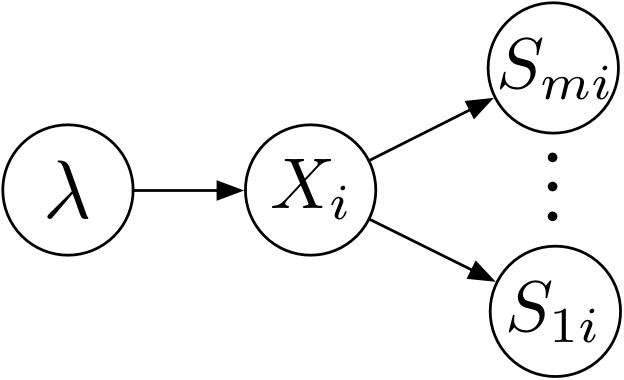
\includegraphics[width=0.6\columnwidth]{./figures/graphical-model.jpg}
\caption{Graphical representation of the partially observable Poisson process.}
\label{fig:gm}
\end{figure}

We obtain a graphical model with the structure shown in Figure~\ref{fig:gm}. There are $m$ sensors polled every sample $i$, $\overrightarrow{s_i}= (s_{1i}, \ldots, s_{mi})$. The true count $x_i$ is a latent variable with posterior inferred from $\overrightarrow{s_i}$, and the posterior of $\lambda$ is inferred from the posterior of $x_i$ after multiple samples $i = 1 \ldots n$.

One way to estimate the parameter $\lambda$ is by Bayesian averaging the posterior  $P(\lambda \mid x_i)$ over all possible count values $x_i$ with mixing proportions equal to the posterior over $x_i$. The posterior of $\lambda$, given $n$ samples $\overrightarrow{s}=(\overrightarrow{s_1} \dots \overrightarrow{s_n})$, each consisting of $m$ sensors, is:
\begin{equation}
	\label{eq:marginal_occurrences}
	\begin{tabular}{r@{=}l}
		$P(\lambda \mid \overrightarrow{s})$ &  $\displaystyle\sum_{x_1=0}^{\infty} \ldots \displaystyle\sum_{x_n=0}^{\infty} P(\lambda \mid \overrightarrow{x}) ~ P(\overrightarrow{x} \mid \overrightarrow{s})$ \\
	\end{tabular}
\end{equation}
\noindent where
\begin{equation*}
	\begin{tabular}{r@{ = }l}
		$P(\lambda \mid \overrightarrow{x})$ & $Gam\Bigg(\lambda \mid \displaystyle\sum_{i=1}^{n} x_i + \alpha, n + \beta \Bigg)$
	\end{tabular}
\end{equation*}
\noindent with $\overrightarrow{x} = (x_1, \ldots, x_n)$ for $1 \leq i \leq n$.

$P(\overrightarrow{x} \mid \overrightarrow{s})$ is factored based on the assumption that each sensor is conditionally independent of the other sensors given $x_i$. Consequently, the probability that the vector of true counts is $\overrightarrow{x}$, given $n$ samples of the vector of $m$ sensed counts $\overrightarrow{s_1}, \ldots, \overrightarrow{s_n}$, is

\begin{equation}
    \label{eq:occurrences_likelihood}
    \begin{tabular}{r@{ $\varpropto$ }l}
        $P(\overrightarrow{x} \mid \overrightarrow{s_1}, \ldots, \overrightarrow{s_n})$ & $P(\overrightarrow{s_1}, \ldots, \overrightarrow{s_n} \mid \overrightarrow{x}) ~ P(\overrightarrow{x})$ \\ [1ex]
        & $\displaystyle\prod_{i=1}^{n} P(\overrightarrow{s_i} \mid x_i) ~ P(x_i)$ \\ [2ex]
        & $\displaystyle\prod_{i=1}^{n} \displaystyle\prod_{j=1}^{m} P(s_{ji} \mid x_i) ~ P(x_i \mid \overrightarrow{x_{-1}})$
    \end{tabular}
\end{equation}

\noindent where $\overrightarrow{x_{-1}} = x_{i-1}, \ldots, x_1$.

$P(x_i \mid \overrightarrow{x_{-1}})$ is calculated in the form of a negative binomial distribution

\begin{equation}
	\label{eq:unconditional_xi}
	\begin{tabular}{r@{=}l}
		$P(x_i \mid \overrightarrow{x_{-1}})$ & $\displaystyle\int_{\lambda=0}^{\infty} P(x_i \mid \lambda) ~ P(\lambda \mid \overrightarrow{x_{-1}}) ~d\lambda$ \\ [2ex]
		& $\displaystyle\int_{\lambda=0}^{\infty} Poi(x_i \mid \lambda) ~ Gam(\lambda \mid \alpha, \beta) ~d\lambda$ \\ [2ex]
		& $NB\Bigg(x_i \mid \alpha, \displaystyle\frac{\beta}{\beta + 1}\Bigg)$
	\end{tabular}
\end{equation}

\noindent and $P(s_{ji} \mid x_i)$ is defined as the aggregate of the true positives $tp_{ji}$ in $x_i$ sub-intervals, and the false positives $fp_{ji}$ in $l-x_i$ sub-intervals. The probability of a TP for sensor $j$ in a sub-interval is $tpr_j = P_j(d = 1 \mid e=1)$, and the probability of an FP is $fpr_j = P_j(d = 1 \mid e=0)$. Thus $P(s_{ji} \mid x_i)$ is defined as a sum of two binomial distributions $B(r \mid n,\pi)$, where the aggregate is constrained to be $s_{ji}$: 

\begin{equation}
	\label{eq:joint_binomial_distribution}
    P(s_{ji} \mid x_i) \! = \! \! \! \displaystyle\sum_{\textrm{tp}_{ji} = 0}^{x_{i}} \! \! B\Big(\textrm{tp}_{ji} \mid x_i, \textrm{tpr}_j\Big) B\Big(\textrm{fp}_{ji} \mid \Delta x_i, \textrm{fpr}_j \Big)
\end{equation}
\noindent where $s_{ji} = \textrm{tp}_{ji} + \textrm{fp}_{ji}$, $\textrm{tpr}_j = P_j(d=1 \mid e=1)$, $\textrm{fpr}_j = P_j(d=1 \mid e=0)$, and $\Delta x_i = (l - x_i)$.

Eqn.~\ref{eq:marginal_occurrences} shows the difficulty of belief state estimation in a POPP since there is no conjugate density. Each sensed count $\overrightarrow{s_i}$ sample used to update the posterior of $\lambda$ adds a factor of countably infinite number of elements. The resulting posterior is a sum of countably infinite sums. One can place an upper bound $l$ on the maximum value of each $x_i$, but it still makes the number of elements in the posterior grow by a factor $l$ with every sensed count $\overrightarrow{s_i}$.  

With this difficulty noted, Jovan et al., proposed three efficient estimators, each of which offers an approximation to the true posterior $P(\lambda \mid \overrightarrow{s})$. A more detailed presentation of these estimators is given in \cite{jovan18a}.
